
\section{Simulation Control}
\label{SimulationControl:sec}

This section describes the different devices which an application may
use to control the simulation. These include {\it control panels} to
allow for the interactive adjustment of properties, {\it controllers}
and {\it input probes} to supply and modify input parameters at the
beginning of each time step, and {\tt monitors} and {\it output
probes} to observe and record simulation results at the end of each
time step.

\subsection{Control Panels}

A {\it control panel} is an editing panel that allows for the
interactive adjustment of component properties.

It is always possible to adjust component properties through the GUI
by selecting one or more components and then choosing {\sf Edit
properties ...} in the right-click context menu. However, it may be
tedious to select the required components, and the resulting panels
present the user with {\it all} properties common to the selections.
A control panel allows an application to provide an editing panel for
a customized set of properties.

\subsubsection{General principles}

Control panels are implemented by the model component
\javaclass[artisynth.core.gui]{ControlPanel}. They can be created and
added within a model's {\tt build()} method by creating an instance of
{\tt ControlPanel}, populating it with widgets for editing the desired
properties, and then adding it to the root model using the {\tt
RootModel}'s
\javamethod*[artisynth.core.workspace.RootModel]{addControlPanel()}
method.

One of the most commonly used means of adding widgets to a control
panel is the method
\javamethodAlt{artisynth.core.gui.ControlPanel.addMethod(HasProperties,String)}%
{addWidget(comp,propertyPath)}, which creates a widget for a property
specified by {\tt propertyPath} with respect to a particular component
{\tt comp}.  Property paths are discussed in the Section
\ref{PropertyHandlesAndPaths:sec}, and can consist simply of a
property name, or, for properties located in descendent components, a
component path followed by a colon '{\tt :}' and a property name.

Other flavors of {\tt addWidget()} also exist, as described in the API
documentation for \javaclass[artisynth.core.gui]{ControlPanel}.  In
addition to property widgets, any type of {\tt Swing} or {\tt awt}
component can be added to a control panel using the method
\javamethodAlt{artisynth.core.gui.ControlPanel.addMethod(Component)}%
{addWidget(awtcomp)}.

Control panels can also be created interactively using the GUI; see
the section "Control Panels" in the
\href{http://www.artisynth.org/doc/html/uiguide/uiguide.html}{
ArtiSynth User Interface Guide}.

\subsubsection{Example: Creating a simple control panel}

\begin{figure}[t]
\begin{center}
\iflatexml
 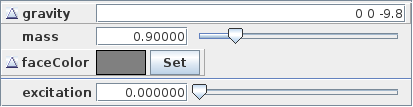
\includegraphics[]{images/controlPanel}
\else
 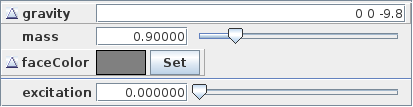
\includegraphics[width=3in]{images/controlPanel}
\fi
\end{center}
\caption{Control panel created by the model {\tt SimpleMuscleWithPanel}.}
\label{controlPanel:fig}
\end{figure}

An model showing a control panel is defined in
%
\begin{verbatim}
  artisynth.demos.tutorial.SimpleMuscleWithPanel
\end{verbatim}
%
This model simply extends {\tt SimpleMuscle} (Section
\ref{SimpleMuscleExample:sec}) to provide a control panel for
adjusting gravity, the mass and color of the box, and the muscle
excitation. The class definition, excluding {\tt include} statements,
is shown below:
%
\lstset{numbers=left}
\begin{lstlisting}
public class SimpleMuscleWithPanel extends SimpleMuscle {
   ControlPanel panel;

   public void build (String[] args) throws IOException {

      super.build (args);

      // add control panel for gravity, rigod body mass and color, and excitation
      panel = new ControlPanel("controls");
      panel.addWidget (mech, "gravity");
      panel.addWidget (mech, "rigidBodies/box:mass");
      panel.addWidget (mech, "rigidBodies/box:renderProps.faceColor");
      panel.addWidget (new JSeparator());
      panel.addWidget (muscle, "excitation");

      addControlPanel (panel);
   }
}
\end{lstlisting}
\lstset{numbers=none}
%
The {\tt build()} method calls {\tt super.build()} to create the model
used by {\tt SimpleMuscle}. It the proceeds to create a {\tt
ControlPanel}, populate it with widgets, and add
it to the root model (lines 8-15). The panel is given the name {\tt
"controls"} in the constructor (line 8); this is its component name
and is also used as the window title for the panel itself. A control
panels does not need to be named, but if it is, then that name must be
unique among the control panels.

Lines 9-11 create widgets for three properties located relative to the
{\tt MechModel} referenced by {\tt mech}. The first is the {\tt
MechModel}'s {\tt gravity}. The second is the {\tt mass} of the box,
which is a component located relative to {\tt mech} by the path name
(Section \ref{PathNames:sec}) {\tt rigidBodies/box}. The third is the
box's face color, which is a sub-property of the box's {\tt
renderProps} indicated by the string {\tt renderProps.faceColor}.

Line 12 adds a {\tt JSeparator} to the panel, using the {\tt
addWidget()} method that accepts general components, and line 13 adds
a widget to control the {\tt excitation} property for {\tt muscle}.

\begin{sideblock}
It should be noted that there are different ways to specify target
properties in {\tt addWidget()}. First, component paths may contain
numbers instead of names, and so the box's mass property could be
specified using {\tt "rigidBodies/0:mass"} instead of {\tt
"rigidBodies/box:mass"} since the box's number is 0. Second, if a
reference to a sub-component is available, one can specify properties
directly with respect to that instead of indicating the sub-component
in the property path. For example, if the box was referenced by a
variable {\tt body}, then one could use the construction
%
\begin{verbatim}
   panel.addWidget (body, "mass");
\end{verbatim}
%
in place of 
%
\begin{verbatim}
   panel.addWidget (mech, "rigidBodies/box:mass");
\end{verbatim}
%
\end{sideblock}

To run this example in ArtiSynth, select {\sf All demos > tutorial >
SimpleMuscleWithPanel} from the {\sf Models} menu. The properties 
shown in the panel can be adjusted interactively by the user,
while the model is either stationary or running.
% SimpleMuscleWithPanel

\subsection{Custom properties}
\label{CustomProperties:sec}

\subsubsection{Adding custom properties to a RootModel}

\subsubsection{Example: a visibility property}

% SimpleMuscleWithProperties

\subsection{Controllers and monitors}

\subsubsection{Purpose and operation}

\subsubsection{A controller to move a point}

% SimpleMuscleWithController

\subsection{Probes}

\subsubsection{Input and output probes}

\subsubsection{Adding probes in code}

% SimpleMuscleWithProbes

\subsubsection{Probe data files}

\subsubsection{Adding probe data in-line}
